\section{Safety - A Method}
Risk, according to ISO 31000\cite{ISO31000}, is the effect of uncertainty on objectives. 
Therefore, in order to minimise risk we need to minimise uncertainty. 

In practical terms this means analysing the system from the top down,
creating a hierarchy of risks to ensure that all issues are considered. 
Taking this approach means that even if the engineer does not identify
every possible cause of failure (which is very likely), mitigation of the
failure modes not identified may still be achieved via global mitigations 
which are applied to an entire branch of the taxonomy. 
When applying a divide and conquer approach as shown in figure\ref{FailTree} we only need
to ensure that each failure set is equal to the union of those below it.

\begin{figure*}[!ht]
  \caption{A hierarchy of failures.}
  \label{FailTree}
  \centering
    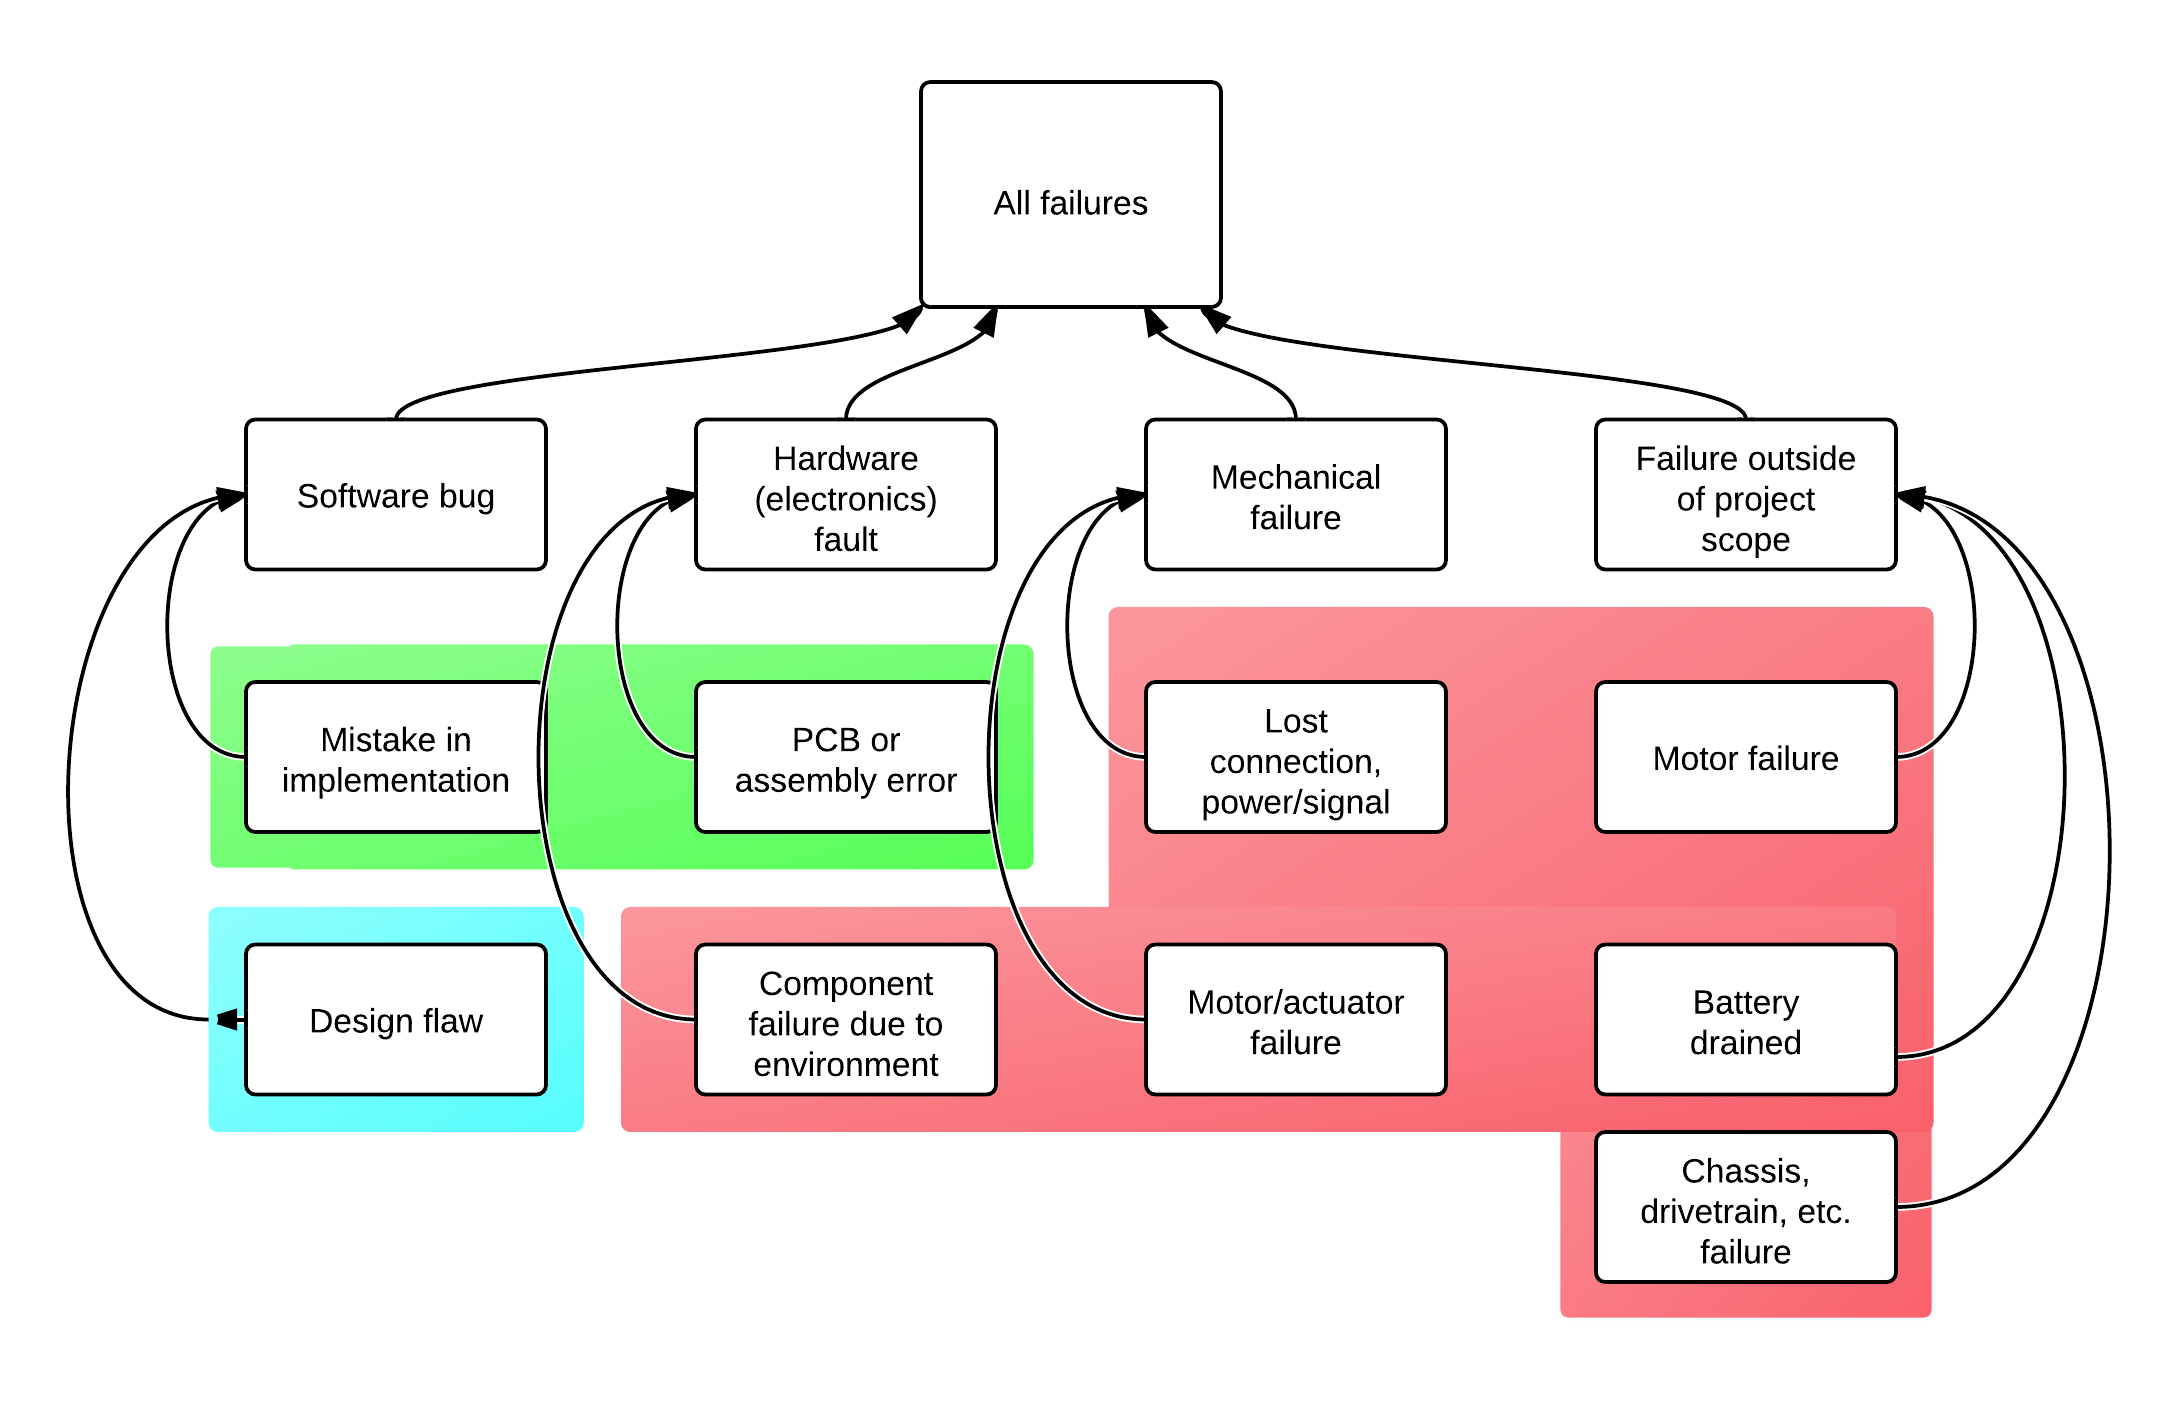
\includegraphics[width=\textwidth]{FailTree}
\end{figure*}

At the lowest level of figure\ref{FailTree} the categories are colour coded into the following groups:

\begin{itemize}
\item[G] Failures that are not a source of risk as they may be eliminated
during testing.
\item[R] Failures that are not preventable but may warrant mitigation.
\item[B] A failure which could happen unpredictably and could be more severe
than loss of power. Preventing this from occurring is the main focus of this paper.
\end{itemize}

\subsection{Preventing Mistakes (Green)}
For a detailed look into software and systems engineering practices see 
Looman's \emph{Software Engineering in the Mariokart System}\cite{
Software Engineering in the Mariokart System}. If standard design practices
such as unit testing are followed then it is possible to eliminate risk from these sources. 

\subsection{Risk Analysis (Red)}


Project managementy stuff

 Full description of all possible failure modes
 
\subsection{Pitfalls in Risk Management}
relying on qualitative judgement

Checking after vs integrated into design



\subsection{Mitigation}
Results of previous section

Global mitigations

Specific mitigations

Un-mitigated risk?

\subsection{Automated model checking to prevent design errors (Blue)}
While it is a given that a structural engineer will calculate forces and stress before
starting constructing and that a mechanical engineer may likewise simulate loads
on his or her design using a CAD package. Software engineering has,
due to the relative flexibility of the medium, been exempt from the expectation
 that a design must be proven before it is implemented. This is not 
 necessarily an advantage, however, as modelling can provide benefits
 including but not limited to proof of system robustness.

SPIN is an automated model checker for `the formal verification of
distributed software system.'\cite{spinroot} The name is an acronym for
Simple Promela INterpretor where Promela is the language used to 
specify a model and its constraints. For more information on SPIN and
Promela visit spinroot.com but for the purposes of this paper an in-depth
knowledge is not required.

When modelling a software system, heavy-handed abstraction is useful
and sometimes necessary. This is because accurately modelling the software
to the level of calculations that have no effect on the system state only 
serves to increase the state-space and therefore the amount of computation
required to check the model. 

Conversely too much abstraction will limit the usefulness of a model to 
being little more than a way of sketching out the top level design of a 
distributed system.

Hence we wish to find an optimal level of detail  which will lie somewhere between the overly 
naive and ultimately useless model which assumes too much; and the result
of several years of work and many hours of computation which simulates
a system down to the instruction set level. 

The level of detail which is right for a project is subject to the law of diminishing
returns, where an increase in the severity of failure or the resources available to
the project will justify a more in depth model to be developed.

  ▲
▲▲
\subsubsection{The (other) Benefits of Modelling a Distributed System}
The obvious aim of modelling is model checking, proving that a design is
correct. 
Promela model vs state diagrams and other sketched plans - or both. iSpin will
 generate sequence diagrams to help visualise process execution.

\subsection{Modelling Mariokart}
A focus on message passing and states.

Unexpected behaviour (errors and power loss) are explicitly specified instead of 
a fine-grained model in which these may arise naturally.

Explain the never claim. plus the automatically generated claims.


\section{Discussion}
A responsible engineer evaluates his design before implementing it and it is the author's opinion 
that this is belief is sometimes lacking in software development. Since a Promela model skips
the details of implementation it is simple to write and understand and does not bury the top level design 
in details. If written beforehand or concurrently then it simplifies writing the software proper
as the design is already specified and proven.

Balancing the cost of Modelling with the benefits it can bring. At what level of detail is it no longer worth 
exploring - dependence on project budget and magnitude of risk outcomes. Focus on projects similar to
Mariokart (ie ones I have experience in).

\section{Conclusion}
